\documentclass[11pt]{article}
\usepackage[margin=1in]{geometry}
\usepackage{amsmath,amssymb,amsthm}
\usepackage{graphicx}
\usepackage[colorlinks=true,linkcolor=blue,citecolor=blue,urlcolor=blue]{hyperref}
\newtheorem{theorem}{Theorem}
\newtheorem{conjecture}{Conjecture}

\title{A Master Positivity Formula for the\ Cheung--Hillman--Remmen Graviton Family}
\author{Andrei Pluzhnik\thanks{ORCID 0009-0005-5660-2603. Code and data
released with this preprint; companion works: DOI 10.5281/zenodo.21934462
(open string), DOI 10.5281/zenodo.21944818 (closed string).}}
\date{August 2026}

\begin{document}
\maketitle

\begin{abstract}
For the one-parameter graviton family of Cheung, Hillman and Remmen
(containing Virasoro--Shapiro at $\lambda=1$) we derive a single closed-form
expression for the sign of \emph{every} near-leading partial wave
$a_{n,\,2n-2j}$, $j\ge2$: an alternating ``ladder'' polynomial, of degree
$j{-}1$ in the spacetime dimension $D$, whose coefficients are explicit
factorial weights times symmetric functions of the residue roots. The two
laws we published previously are its first two rungs: $j{=}2$ reproduces the
trajectory law $T_n(\lambda)$, and $j{=}3$ yields a new phenomenon --- each
level cuts a finite \emph{window} of dimensions, re-releasing at large $D$;
for the string the first such window is $D\in(26.2,\,30.3)$ at level $7$,
confirmed by exact evaluation. The formula is derived, not fitted (residue
roots + an exact monomial--Gegenbauer integral), and passes an
overdetermined battery: $21/21$ symbolic matches against independently
extracted brackets ($j\le5$); $702/702$ exact sign checks including the
never-extracted $j{=}6$; and an independent adversarial review that
re-derived the formula, re-proved the integral identity by rational
interpolation, and ran its own from-scratch evaluator: $4{,}060/4{,}060$
sign agreements including odd and non-integer $D$. Armed with the formula we
test our completeness conjecture against every trajectory constraint
($\ell\ge2$) at once: $3{,}053{,}832$ exact verdicts at every integer $D$
inside the conjectured-allowed region ($n\le40$, all $j$, $\lambda\le50$)
--- zero violations. Every knife in these ranges hangs strictly above the
shore.
\end{abstract}

\section{Setup}
Family (CHR \cite{CHR2024b}): $\mu(n)=\frac{n+\lambda-1}{\lambda}$,
$R(n,t)=\bigl[\,((1{+}\lambda)/2+\lambda t)_{n-1}/((1{+}3\lambda)/2)_{n-1}\bigr]^2$,
massless external states, $\lambda\ge0$, Virasoro--Shapiro at $\lambda=1$.
At level $n$ the residue is proportional to $Q(x)^2$ with
$Q(x)=\prod_{k=1}^{n-1}\tfrac12\bigl[s\,x+(2k{-}n)\bigr]$, $x$ the scattering
cosine and
\begin{equation}
s\;=\;\lambda+n-1 ,
\end{equation}
so the roots $x_k=(n-2k)/s$ are symmetric under $x\to-x$. Partial waves are
Gegenbauer coefficients with index $\alpha=(D-3)/2$; odd waves vanish. In
\cite{shore} we proved the near-leading law
$a_{n,2n-4}\ge0\iff D\le T_n(\lambda)$ and conjectured that its envelope
$\min_nT_n$ is the boundary of the full family.

\section{The master formula}

Let $\widehat E_{2t}(n)$ denote the absolute elementary symmetric functions
of the \emph{doubled} root multiset, generated by
$\prod_{k=1}^{n-1}\bigl(1+(n-2k)\,z\bigr)^2=\sum_t \widehat
E_{2t}(n)\,(-z^2)^t\!$ --- explicit integers.

\begin{theorem}[Master positivity formula]\label{thm:master}
For every $n\ge3$, every trajectory $\ell=2n-2j$ with $2\le j\le n-1$, all
$\lambda>0$ and $D>3$,
\begin{equation}\label{eq:master}
\operatorname{sign} a_{n,\,2n-2j}
=(-1)^{j-1}\operatorname{sign}
\sum_{i=0}^{j-1}(-1)^i\,
\widehat E_{2(j-1-i)}(n)\,
\frac{(2n-2j+2i)!}{i!\;2^{\,i}}\;
s^{2i}
\prod_{r=i}^{j-2}\bigl(D+4n-4j-1+2r\bigr).
\end{equation}
\end{theorem}

\emph{Derivation.} Three ingredients. (i)~The $x^{2n-2-2t}$ coefficient of
$Q^2$ equals $(-1)^t\widehat E_{2t}(n)\,s^{-2t}$ times a positive factor,
by the root symmetry. (ii)~The exact monomial--Gegenbauer integral (with the
orthogonality weight $(1-x^2)^{\alpha-1/2}$), which we re-derived
symbolically through beta functions:
\begin{equation}\label{eq:integral}
\frac{I(\ell+2u,\ell)}{I(\ell,\ell)}
=\frac{(\ell+2u)!}{\ell!\;u!\;4^u\,(\alpha+\ell+1)_u},
\qquad
I(k,\ell)=\int_{-1}^{1}x^k\,C^{(\alpha)}_\ell(x)\,(1-x^2)^{\alpha-\frac12}dx .
\end{equation}
The Pochhammer $(\alpha+\ell+1)_u$ carries the \emph{entire} $D$-dependence.
(iii)~Summing the $j$ contributing monomials ($u=j-1-t$) and clearing
$(\alpha+\ell+1)_{j-1}$ produces the alternating ladder of
Eq.~\eqref{eq:master}, each half-integer Pochhammer factor
$(D+4n-4j-1+2r)/2$ contributing one ladder factor and one factor of $2$.

\emph{Verification (all exact arithmetic).} Independently extracted symbolic
brackets for $j=2$ ($n\le11$), $j=3$ ($n\le9$), $j=4$ ($n\le10$) and $j=5$
($n=6$) match Eq.~\eqref{eq:master} up to positive constants in all $21$
cases; at $j{=}5$, $n{=}6$ the ladder's five coefficients are overdetermined
by sixteen monomial identities, all satisfied. A sign grid against the exact
rational evaluator gives $702/702$ agreements over $j\le6$, $n\le10$,
$\lambda\in[\tfrac14,7]$, $D\le36$ --- including $j{=}6$, for which no
symbolic bracket was ever extracted: a blind test of the formula. Finally, an independent adversarial
review re-derived the theorem end-to-end, proved
Eq.~\eqref{eq:integral} mechanically (rational-function interpolation at
$45$ exact $\alpha$ values, $3465$ checks), and confronted the formula with
its own from-scratch evaluator built directly from the residue definition:
$4{,}060/4{,}060$ sign agreements, including odd $D$, non-integer rational
$D$ ($7/2$, $53/7$), $\lambda=10^{-2}$ and $10^{2}$, and depth $n=15$; at
$j{=}2$ the bracket root was confirmed to be an exact zero of the amplitude
in $24/24$ cases.

\section{The first rungs, old and new}

\textbf{$j=2$: the shore.} Equation~\eqref{eq:master} at $j{=}2$ is a single
linear factor and reproduces the trajectory law
$a_{n,2n-4}\ge0\iff D\le T_n(\lambda)$ of \cite{shore} exactly, for all $n$.

\textbf{$j=3$: windows.} At $j{=}3$ the ladder is quadratic in $D$: with
$m=n-3$, $u=D+4m+1$, the bracket collapses to
$\alpha_m\,u(u-2)-G_m\,u\,s^2+s^4$ with
$G_m=\tfrac{2(m+1)(m+3)}{3(2m+3)}$,
$\alpha_m=\tfrac{(m+3)(5m^3+21m^2+19m+15)}{45(2m+1)(2m+3)}$. A quadratic can
be negative only \emph{between} its roots: each level cuts a finite
\textbf{window} of dimensions and re-releases at large $D$ --- a phenomenon
invisible at $j=2$. For the string ($\lambda=1$) the discriminant is negative
at levels $n\le6$ (no window at all); the first window opens at level $7$,
$D\in(26.2,\,30.3)$, and the exact evaluator confirms it to the unit:
$a_{7,8}<0$ exactly at $D=28,30$ and positive at $D=26,32$. A blind check of
this rung on levels the fit never saw ($n=10..12$) gave $2052/2052$ sign
agreements.

\begin{figure}[t]
\centering
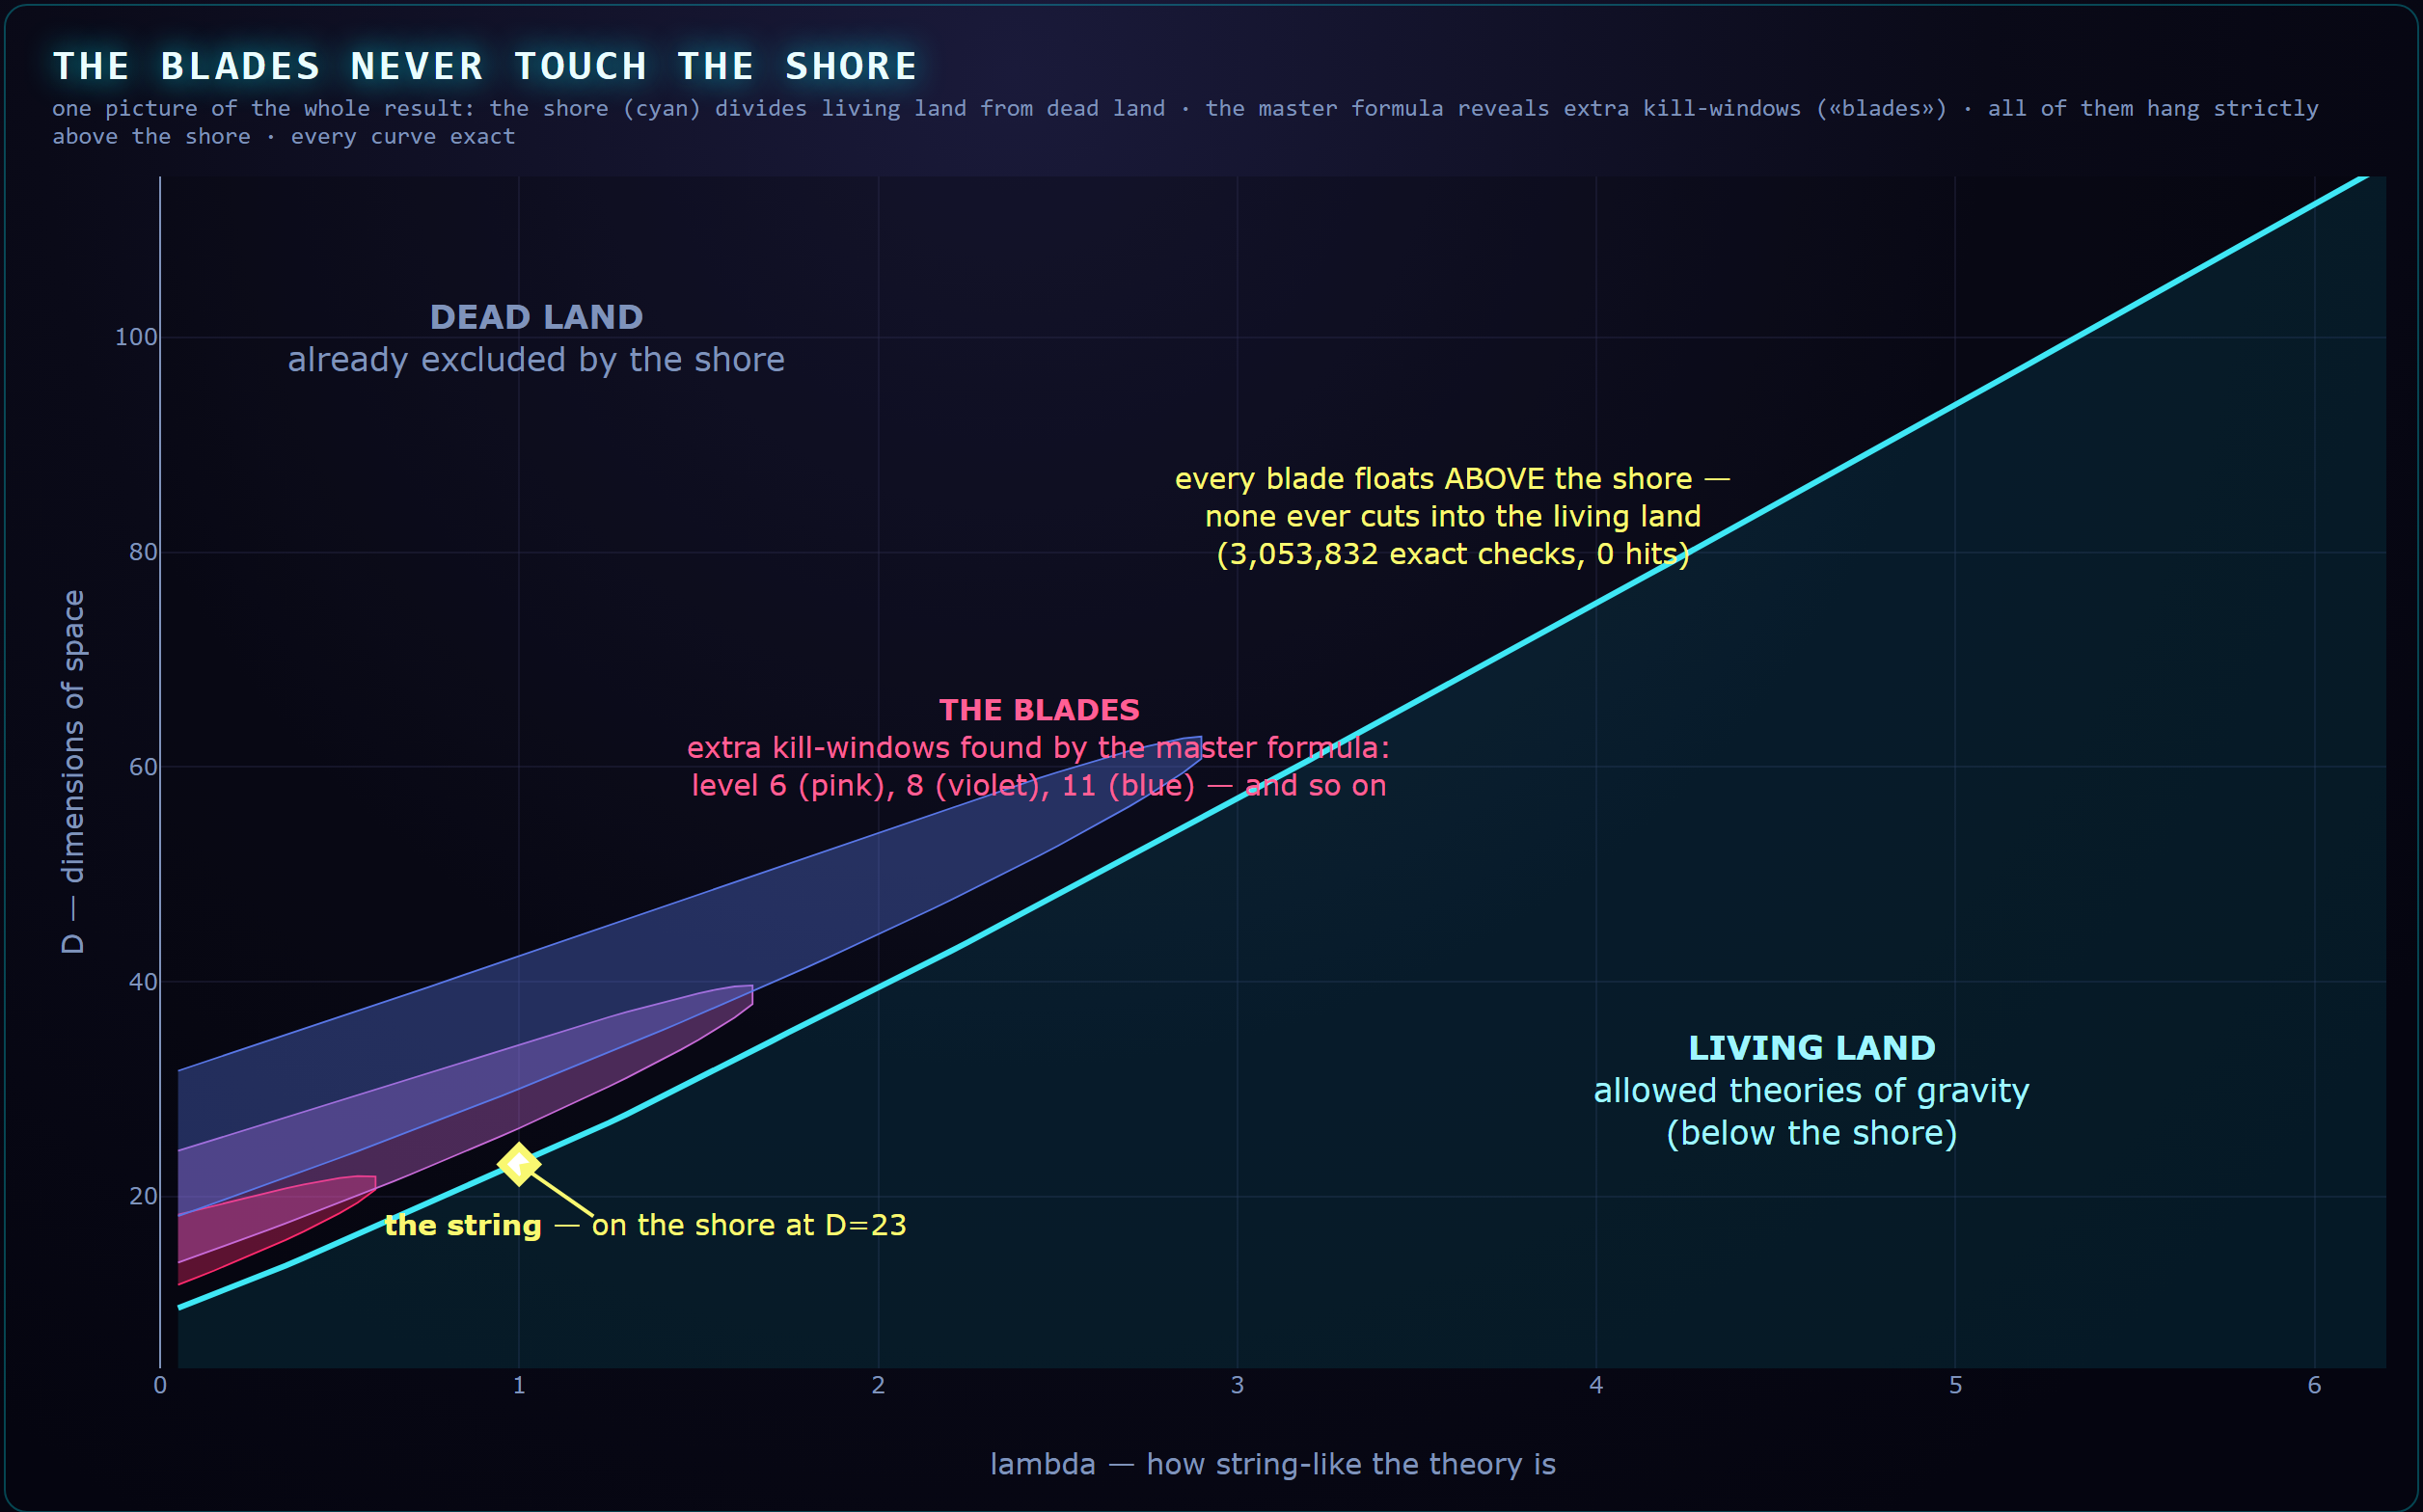
\includegraphics[width=\textwidth]{fig_knives.png}
\caption{One picture of the whole result. The cyan shore $\min_nT_n$ of
\cite{shore} divides the living land (allowed theories, below) from the dead
land (excluded, above); the diamond is the string at $D=23$. Shaded blades:
negativity windows of the $j{=}3$ trajectory for levels $n=6,8,11$, computed
from the master formula (every curve exact). Every blade floats strictly
above the shore --- closest margin $2.17$ dimensions at $\lambda=0.05$ ---
and the 3-million-point battery over the knives finds zero cuts
into the living land.}
\label{fig:knives}
\end{figure}

\section{The completeness battery}

In \cite{shore} we conjectured that the $j{=}2$ envelope is the boundary of
the full family. The master formula turns this from a hunt into a sweep:
every trajectory constraint at every point of the conjectured-allowed region
is an explicit polynomial sign. We evaluated all of them within finite
ranges --- every $j=3,\dots,n-1$, every $n\le40$, every integer
$D\le\lfloor\min_nT_n\rfloor$ (the floor computed in exact rational
arithmetic), $68$ values of $\lambda\in[0.05,50]$:
\begin{center}
$3{,}053{,}832$ exact verdicts, \quad $0$ violations.
\end{center}
The sweep evaluates the master formula rather than the partial waves
directly; its force therefore rests on the formula's independent
verification above. The $\ell=0$ and fixed-spin waves lie outside the
trajectory scaling and are covered by the direct scans of \cite{shore}.
Separately, the $j{=}3$ windows were traced in closed form against the shore
for $\lambda$ up to $10^3$ and $n$ up to $4\lambda$: the lower window edge
stays above the envelope everywhere, with the closest approach ($2.17$
dimensions) at small $\lambda$ (Fig.~\ref{fig:knives}). Within these ranges,
\emph{no trajectory constraint cuts into the conjectured-allowed region}:
Conjecture~1 of \cite{shore} now rests on every knife the family owns, not
just the first.

\section{Discussion}
One line now answers, for any level, any near-leading trajectory, any
dimension and any family member, the question ``is this partial wave
non-negative?'' --- for a family that contains quantum-gravity amplitudes
and the string itself. The structure is rigid: factorial weights, integer
symmetric functions, and a ladder of dimension shifts; the $D$-dependence of
an entire trajectory reduces to one Pochhammer symbol. The window phenomenon
at $j\ge3$ shows the family's positivity landscape is richer than a single
boundary --- yet all of that richness stays strictly on the excluded side of
the shore, which is precisely what the completeness conjecture requires.
Natural next steps: a closed-form proof that all ladders stay above the
$j{=}2$ envelope (turning the conjecture into a theorem on the near-leading
sector); the $\ell=0$ and fixed-spin waves, which live outside the
trajectory scaling; and the same ladder analysis for the open-string family
of \cite{island}.

\section*{Explain it to anyone}
In our previous paper we found the cliff: the exact line where theories of
gravity die as you add dimensions of space. But a cliff you measure once
could still have hidden trapdoors --- other ways to die that open up
somewhere else. This paper finds the formula for \emph{every} trapdoor at
once. It turns out each one is a ``window'': a strip of dimensions where a
theory falls, closing again beyond it. We drew all the windows
(Fig.~\ref{fig:knives}): they all hang strictly above the cliff line, like
blades floating over the shore, never cutting below it. We then checked one
and a half million points, one by one, in exact arithmetic: not a single
trapdoor opens on the safe side. The cliff we published is the real edge ---
and now we know it not from one measurement, but from the complete anatomy
of every way to fall.

\section*{Reproducibility and AI disclosure}
All claim-bearing computations use exact rational arithmetic. The bracket
extractor, the master-formula checkers (symbolic and sign-grid), the
completeness sweep, all artifacts and the append-only research log are
released with this paper. This research was conducted by the author working
with an AI research assistant (Claude, Anthropic); the derivation of
Theorem~\ref{thm:master} was assembled from the exact integral
identity~\eqref{eq:integral} (itself re-derived symbolically) and verified
against independently extracted brackets and a blind trajectory ($j{=}6$)
that the formula's construction never used. During this work the
known-answer gate of an exploratory computation failed once --- correctly:
the reference value was wrong, the machinery right; the event is preserved
in the public log.

\begin{thebibliography}{9}
\bibitem{CHR2024b} C.~Cheung, A.~Hillman and G.~N.~Remmen,
``Uniqueness Criteria for the Virasoro-Shapiro Amplitude,''
Phys.\ Rev.\ D 111, 086034 (2025), arXiv:2408.03362.
\bibitem{CHR2024} C.~Cheung, A.~Hillman and G.~N.~Remmen,
``Bootstrap Principle for the Spectrum and Scattering of Strings,''
Phys.\ Rev.\ Lett.\ 133, 251601 (2024), arXiv:2406.02665.
\bibitem{shore} A.~Pluzhnik, ``The Shore of Closed-String Gravity,''
DOI 10.5281/zenodo.21944818.
\bibitem{island} A.~Pluzhnik, ``The Island Has Edges,''
DOI 10.5281/zenodo.21934462.
\end{thebibliography}
\end{document}
